\documentclass[10pt,twocolumn]{article}
\usepackage[margin=0.75in,columnsep=0.28in]{geometry}
\usepackage{graphicx}
\usepackage{booktabs}
\usepackage{amsmath}
\usepackage{xcolor}
\usepackage{listings}
\usepackage[font=small,labelfont=bf]{caption}
\usepackage{microtype}
\usepackage[hidelinks]{hyperref}
\usepackage{titlesec}
\titlespacing*{\section}{0pt}{1.1ex plus .3ex}{.6ex}
\titlespacing*{\subsection}{0pt}{.9ex plus .2ex}{.4ex}

\lstset{language=C,basicstyle=\ttfamily\scriptsize,columns=fullflexible,keepspaces=true,
  frame=single,framerule=0.3pt,rulecolor=\color{black!30},aboveskip=4pt,belowskip=2pt,
  commentstyle=\color{black!55}\itshape,keywordstyle=\bfseries,numbers=none,xleftmargin=2pt}

\newcommand{\mcssp}{\textsc{MCS-SP}}

\title{\vspace{-1.2em}\textbf{Scalable Spin Locks and Barriers on a Modern Hybrid Multicore:\\
Reproducing Mellor-Crummey \& Scott (1991) and Making MCS Preemption-Tolerant}\vspace{-0.4em}}
\author{Course: Multicore Architecture and Programming --- Research Paper Assignment}
\date{\vspace{-0.6em}November 2026\vspace{-0.8em}}

\begin{document}
\maketitle

\begin{abstract}
\noindent
Mellor-Crummey and Scott's 1991 paper introduced the MCS queue lock and showed that busy-wait
synchronization need not cause memory contention if every waiter spins on its own local flag. We
re-implement the paper's five spin locks and three of its barriers in portable C11 and re-run its
experiments 35 years later on a hybrid 12-thread Intel Core i7-1255U. While threads do not outnumber
cores, the paper's conclusions hold. The queue locks scale with near-perfect fairness, test-and-test\_and\_set
does not, and MCS keeps its modest premium in uncontended latency. Modern hardware also changes two things.
Unfair locks now look 5--10$\times$ faster on the paper's own metric simply by keeping the lock in one
cache, and the dissemination barrier, not the centralized one, is fastest. The paper's acknowledged weakness,
FIFO locks under preemption, dominates on a shared machine: with 2--4$\times$ more threads than hardware threads, MCS
slows down by up to 1500$\times$ and starves threads. We propose \mcssp{}, a spin-then-park MCS lock
(about 20 extra lines, futex-based) that keeps FIFO order and MCS's cost when undersubscribed. When
oversubscribed it delivers 9--29$\times$ more throughput than MCS and uses 25--70$\times$ less CPU. A second
step, wake-ahead, lifts strict FIFO to glibc-mutex throughput near saturation. We also quantify the remaining gap
to barging locks as the inherent price of FIFO hand-off to sleeping threads.
\end{abstract}

\section{Introduction}
Every shared-memory parallel program eventually waits: for a lock to become free, or for
other threads to reach a barrier. How a thread waits decides whether the program scales. A
naive spin lock makes every waiting core hammer the same memory word. That turns the cache-coherence
interconnect into a serial bottleneck and can make adding cores \emph{slow the program down}.

Mellor-Crummey and Scott's 1991 paper~\cite{mcs91} showed that this contention is
not fundamental. Their key idea is that \emph{every processor should spin on its own, locally
accessible flag, and some other processor should end the spin with a single remote write}. They built
the MCS queue lock and a tree barrier on this principle, and compared them with the other spin
locks and barriers known at the time. The comparison ran on a bus-based Sequent Symmetry and on a BBN
Butterfly, a machine without coherent caches. The paper won the 2006 Dijkstra Prize. Its lock lives on
inside the Linux kernel's \texttt{qspinlock}~\cite{qspinlock}, and its local-spinning principle is
textbook material~\cite{amp}.

This report does three things:
\begin{enumerate}\setlength\itemsep{0pt}
\item \textbf{Implementation.} We implement the paper's five spin locks (Algorithms 1, 2, 3, 5 and 6) and
three of its barriers (Algorithms 7, 9 and 11) in portable C11 with explicit memory orderings. We add
naive baselines, the glibc primitives, and a cache-padding ablation.
\item \textbf{Replication.} We re-run the paper's style of experiment on a 2022 Intel Core i7-1255U
laptop CPU. This CPU is a \emph{hybrid} multicore with 2 performance and 8 efficiency cores, giving 12
hardware threads. We ask which of the 1991 conclusions still hold 35 years later.
\item \textbf{Extension.} The paper itself warns that its FIFO locks ``waste CPU resources if spinning
processes may be preempted'' (\S4.3). It recommends falling back to a test\_and\_set lock in that
case, giving up fairness. We propose \mcssp{}, a \emph{spin-then-park} MCS lock that keeps FIFO order
and local spinning but parks waiters in the kernel (Linux \texttt{futex}) after a bounded spin. We show
that it removes MCS's collapse when threads outnumber cores, at no cost when they do not. We apply the
same principle to the centralized barrier.
\end{enumerate}

\section{Background: the original paper}
\label{sec:background}
\paragraph{The problem.} On a cache-coherent machine, a lock word that many cores read and write
bounces between their caches. Every release then invalidates every waiter's copy, and every waiter
re-fetches the line, so each hand-off costs $O(P)$ coherence traffic for $P$ waiters. On a machine
without coherent caches, such as the Butterfly, spinning on a remote word saturates the network outright.

\paragraph{Locks studied (paper \S2).}
\textbf{Alg.~1}, test\_and\_set with exponential backoff: waiters back off for doubling delays to thin out
traffic, but the lock is unfair. \textbf{Alg.~2}, the ticket lock with proportional backoff:
\texttt{fetch\_and\_increment} hands out tickets, which gives FIFO order. A waiter delays in proportion to how
many tickets are ahead of it, but everyone still polls one shared \texttt{now\_serving} word.
\textbf{Alg.~3}, Anderson's array lock~\cite{anderson90}: each waiter spins on its own array slot,
so traffic is local, but space is $O(P)$ per lock. \textbf{Alg.~4}, Graunke and Thakkar's
lock~\cite{gt90}, is a similar array lock (we do not implement it).

\paragraph{The MCS lock (Alg.~5).} The lock is a single \texttt{tail} pointer to a queue of per-thread
nodes. To acquire, a thread atomically swaps its own node into \texttt{tail}. If there was a
predecessor, the thread links itself behind it and spins on the \texttt{locked} flag \emph{in its own
node}. To release, the holder clears its successor's flag, which is one remote write. If it has no
successor yet, it uses \texttt{compare\_and\_swap} to reset \texttt{tail}. The lock takes $O(1)$ space
per lock plus one node per thread, $O(1)$ remote references per acquisition, and gives FIFO order.
\textbf{Alg.~6} releases with \texttt{fetch\_and\_store} only, for machines without CAS, at the price
of rare out-of-order ``usurpers''.

\paragraph{Barriers (paper \S3).} \textbf{Alg.~7} is a centralized counter barrier with a
sense-reversing flag. \textbf{Alg.~9} is the dissemination barrier~\cite{hfm88}, which runs
$\lceil\log_2 P\rceil$ rounds of pairwise signalling. \textbf{Alg.~11} is the paper's new tree barrier:
arrival goes up a 4-ary tree and wake-up comes down a binary tree. Each thread spins only on its own
node, and the barrier needs the theoretical minimum of $2P-2$ network transactions on machines without
broadcast. The paper also covers a combining-tree barrier (Alg.~8) and a tournament barrier (Alg.~10),
which we do not implement.

\paragraph{The paper's conclusions.} The recommendations in \S5 are: use MCS if
\texttt{fetch\_and\_store} is available. Use the ticket lock with proportional backoff if
one-processor latency dominates. Use test\_and\_set with capped exponential backoff ``if processes
might be preempted while spinning''. On broadcast-based coherent machines, use a centralized
barrier for modest $P$, and the dissemination or tree barrier otherwise.

\section{Implementation}
\label{sec:impl}
All code is C11 (\texttt{<stdatomic.h>}) plus POSIX threads, about 1\,100 lines. Every lock implements one
vtable (\texttt{create}, \texttt{acquire(lock, ctx)}, \texttt{release(lock, ctx)}). The per-thread context
holds the MCS node and the Anderson slot index, so every lock pays the same indirect-call overhead in the
harness. Table~\ref{tab:locks} lists what we built.

\begin{table}[t]
\centering\small
\caption{Implemented synchronization algorithms.}
\label{tab:locks}
\begin{tabular}{@{}ll@{}}
\toprule
Name & Description \\
\midrule
\texttt{tas\_backoff} & test\_and\_set + exp.\ backoff (Alg.~1)\\
\texttt{ticket} & ticket + proportional backoff (Alg.~2)\\
\texttt{anderson} & array queue lock, padded slots (Alg.~3)\\
\texttt{mcs} & MCS list queue lock (Alg.~5)\\
\texttt{mcs\_swap} & MCS, \texttt{fetch\_and\_store}-only release (Alg.~6)\\
\texttt{tas}, \texttt{ttas} & no-backoff baselines\\
\texttt{anderson\_np} & Alg.~3 without padding (ablation)\\
\texttt{pthread} & glibc \texttt{pthread\_mutex\_t}\\
\textbf{\texttt{mcs\_sp}} & \textbf{spin-then-park MCS (ours, \S\ref{sec:ext})}\\
\textbf{\texttt{mcs\_spw}} & \textbf{\texttt{mcs\_sp} + wake-ahead (ours, \S\ref{sec:wake})}\\
\midrule
\texttt{central} & sense-reversing counter barrier (Alg.~7)\\
\texttt{dissem} & dissemination barrier (Alg.~9)\\
\texttt{mcs\_tree} & 4-ary arrival / binary wake-up tree (Alg.~11)\\
\texttt{pthread} & glibc \texttt{pthread\_barrier\_t}\\
\textbf{\texttt{central\_sp}} & \textbf{spin-then-park central barrier (ours)}\\
\bottomrule
\end{tabular}
\end{table}

\paragraph{From sequential consistency to C11 orderings.} The 1991 pseudocode assumes every memory
access is sequentially consistent. Modern compilers and CPUs reorder freely, so we chose an ordering for
each access. The rule is that a lock hand-off is a \emph{release} store by the old holder that the new
holder reads with an \emph{acquire} load. That creates the happens-before edge which publishes the
critical section's writes. For MCS, the swap on \texttt{tail} is \texttt{acq\_rel}. It must acquire when the lock was
free, since it synchronizes with the last releaser's CAS, and it must release so that the node's
initialisation is visible to a successor. Linking \texttt{pred->next} is a release store. That ensures
our \texttt{locked=1} write is ordered before the releaser's \texttt{locked=0}. Without it, the waiter
could overwrite the grant and spin forever. Spin loads are acquire, and only the final hand-off pays for
ordering. On x86 most of these compile to plain \texttt{mov}s (TSO), but the code is also correct on
Arm.

\paragraph{Faithful-but-modern deviations.}
(i) \emph{Padding.} Every hot word (lock words, MCS nodes, Anderson slots, barrier flags) is aligned to
128\,B, not 64\,B. Intel's adjacent-line prefetcher fetches 64\,B lines in pairs, so two words 64\,B apart
can still interfere. The paper also padded to ``avoid unnecessary invalidations'' on the Symmetry. \texttt{anderson\_np} measures what
padding is worth.
(ii) \emph{Anderson wrap-around.} The paper corrects the slot counter with an extra atomic add. We size the
array to a power of two and let the unsigned counter wrap, which is equivalent and needs one atomic fewer.
(iii) \emph{Tree barrier flags.} Alg.~11 packs the four \texttt{childnotready} flags as four bytes of one word,
and children write them with byte stores. Mixed-size atomics are not portable C11, so children clear a
bit with \texttt{atomic\_fetch\_and}. The parent still spins on one local word.
(iv) \emph{Spin hint.} Every spin loop executes \texttt{PAUSE}, which saves power and avoids memory-order
mis-speculation when the loop exits. Backoff delays are counted in \texttt{PAUSE} iterations. The defaults
are base 1 and cap 1024 for Alg.~1, and 1 per waiter ahead for Alg.~2.

\paragraph{Correctness checking.} Every benchmark run is also a test. The critical section
increments a \emph{plain, non-atomic} counter that only the lock protects, and the run fails unless
it equals the sum of per-thread acquisition counts. The barrier benchmark publishes each thread's episode
number before the barrier and checks after it that peers have reached that episode and are at most one
ahead. \texttt{make test} runs every lock with 1--32 threads and every barrier with 1--24 threads.
All runs in this report passed these checks.

\section{Extension: \mcssp{}}
\label{sec:ext}
\subsection{Motivation}
FIFO hand-off is what makes MCS fair, and it is also its weak point. The releaser \emph{chooses} the next
owner. If that thread is not currently running because it was preempted, or because there are more threads
than cores, the lock is owned by a sleeping thread. Nobody can make progress until the scheduler runs it
again, typically milliseconds later. Meanwhile every other queued waiter spins through its entire time
slice and steals CPU from the very threads that need it, the holder and the next waiter. This
\emph{lock-waiter preemption} turns a lock that costs tens of nanoseconds into one that costs a time slice
per hand-off. Today it is common: a laptop running a browser, an IDE and several AI agents is rarely idle,
cloud vCPUs are time-shared by the hypervisor, and thread pools are routinely sized above the core count.

The paper's answer (\S4.3, \S5) is co-scheduling, or giving up FIFO by switching to
test\_and\_set with backoff, which lets running latecomers barge ahead. We instead keep the queue and change
only \emph{how a waiter waits}.

\subsection{Design}
\begin{lstlisting}
// waiter (after linking behind pred)
for (i = 0; i < spin_limit; i++) {      // phase 1:
  if (load_acq(&me->locked) == 0) return;  // = MCS
  cpu_relax();
}
if (!CAS(&me->locked, 1 -> 2)) return;  // granted meanwhile
while (load_acq(&me->locked) != 0)      // phase 2:
  futex_wait(&me->locked, 2);           //  sleep

// releaser, hand-off to succ
old = exchange_rel(&succ->locked, 0);
if (old == 2) futex_wake(&succ->locked, 1);
\end{lstlisting}
The \texttt{locked} word now has three states: 0 means granted, 1 means waiting and spinning, and 2 means
parked or about to park. A waiter spins exactly as in MCS for up to \texttt{spin\_limit} iterations, which is
1024 \texttt{PAUSE}s by default. If the lock has not arrived, it announces that it is going to sleep with a CAS
from 1 to 2 and blocks in \texttt{futex\_wait}. The releaser replaces MCS's plain store with an atomic
\texttt{exchange}. If the old value was 2, it issues one \texttt{futex\_wake}. When threads $\le$ cores,
the hand-off arrives during phase 1, so no system call is ever made. The only extra cost on that path is
an \texttt{xchg} instead of a \texttt{mov}. The release-side wait for a successor to link itself, which
the paper's code spins on, also yields the CPU after \texttt{spin\_limit} iterations, because the successor
may have been preempted between its swap and its link.

\subsection{Why it is correct}
Mutual exclusion and FIFO order are inherited unchanged from MCS, because the queue manipulation is
identical. What we must show is that \textbf{no wake-up is lost}. There are two cases.
(a) The waiter's CAS $1\to2$ comes before the releaser's exchange in the modification order of
\texttt{locked}. Then the exchange returns 2 and the releaser calls \texttt{futex\_wake}. If the waiter has
not yet entered the kernel, \texttt{futex\_wait(addr, 2)} atomically sees the value is no longer 2 and
returns at once. (b) The exchange comes first. Then the waiter's CAS fails, because it reads 0, and the
waiter owns the lock without ever sleeping. Spurious and late wakes are harmless, because the waiter
re-checks \texttt{locked} in a loop. A late \texttt{futex\_wake} that reaches a node already reused for a
later acquisition only causes one spurious re-check. Nodes are per-thread and never freed while the
benchmark runs, so the wake never touches freed memory.

\subsection{Step 2: wake-ahead (\mcssp{}W)}
\label{sec:wake}
Our first measurements (\S\ref{sec:results}) showed that \mcssp{} removes the collapse. Once waiters are
asleep, though, a strict FIFO lock passes \emph{at most once per wake-up latency} $L$, the time from
\texttt{futex\_wake} until the woken thread is running, which is several microseconds. If the critical
section takes $S \ll L$, the hand-off period is $S+L \approx L$. An unfair lock such as glibc's mutex
avoids this because a thread that is already running barges in. We want the same effect without giving up FIFO.

\mcssp{}W lets the \emph{new holder} walk up to $D$ nodes down the queue (default $D=2$) immediately after
acquiring the lock. It pre-wakes any waiter it finds parked with a CAS $2\to1$ followed by
\texttt{futex\_wake}. A pre-woken waiter sees \texttt{locked}$=1$ and goes back to spinning, and it may park
again. This walk is safe because no node behind the holder can be granted while the holder still holds
the lock: only its own release starts that chain, so every node it reaches is still enqueued and live. If a
pre-wake wins the race against a later release, the releaser's exchange returns 1 and correctly skips the
\texttt{futex\_wake}. In steady state each holder issues about one pre-wake. The $D$ waiters nearest the
head are kept awake, so a wake-up overlaps $D$ critical sections and the period approaches
$\max(S + c_{\text{wake}}, L/D)$. Here $c_{\text{wake}}$ is the cost of the pre-wake system call, which
the holder pays while it holds the lock. That is the trade-off.

\subsection{Relation to prior work}
Spin-then-block (``two-phase'') waiting is an old idea; Karlin et al.\ studied how long to spin before
blocking~\cite{karlin91}. Production mutexes combine bounded spinning with sleeping: glibc's
\emph{adaptive} mutex type spins before its futex sleep~\cite{futex}, and the Linux kernel's \texttt{mutex}
spins optimistically while the owner is running. These are not FIFO queue locks with local spinning, though.
The closest research lines are preemption-adaptive queue locks such as He, Scherer and Scott's
time-published locks~\cite{tp05}. Those let waiters detect preempted peers and \emph{remove} them from the
queue, which is more powerful but needs timestamps and a far more complex protocol. Dice's Malthusian
locks~\cite{malthusian} and the SOSP'19 shuffle locks~\cite{shfl} also park excess waiters. Our goal is
deliberately modest. It is the smallest change to the paper's Alg.~5 that fixes the failure mode the
paper itself identifies: about 20 extra lines for \mcssp{} and 30 more for wake-ahead. Keeping a small set
of waiters near the head awake is close in spirit to the ``active set'' of Malthusian locks, but we never
reorder the queue.

\section{Methodology}
\label{sec:method}
\paragraph{Platform.} The machine is an Intel Core i7-1255U (Alder Lake, 2022). It has 2 performance cores
(P, SMT, up to 4.7\,GHz; logical CPUs 0--3) and 8 efficiency cores (E, no SMT, up to 3.5\,GHz; two clusters
of four, each sharing a 2\,MB L2). All cores share a 12\,MB L3. Software is Fedora Linux 7.3 and gcc 16.2
with \texttt{-O2}. Table~\ref{tab:calib} lists hardware constants we measured with our \texttt{calibrate}
tool. They are the modern counterparts of the paper's ``remote reference'' costs.

\begin{table}[t]\centering\small
\caption{Measured constants (best of 5). ``Line transfer'' is one-way cache-line ping-pong latency
between two pinned threads. ``Futex wake-up'' is one-way \texttt{futex\_wake}$\to$running latency.}
\label{tab:calib}
\begin{tabular}{@{}lr@{}}\toprule
Quantity & Value\\\midrule
\texttt{PAUSE}, P-core / E-core & 49.6 / 24.7\,ns\\
Line transfer, SMT siblings (0--1) & 28\,ns\\
Line transfer, P$\leftrightarrow$P / P$\leftrightarrow$E & 46 / 48\,ns\\
Line transfer, E$\leftrightarrow$E same / other cluster & 61 / 45\,ns\\
Futex wake-up (pinned / unpinned) & 2.4 / 2.8\,$\mu$s\\\bottomrule
\end{tabular}
\end{table}

\paragraph{Workloads and metrics.} We follow the paper's method (\S4.2): each thread acquires and
releases the lock in a tight loop. The \emph{empty} workload only increments the protected counter, as in
the paper's Figs.~4--6. The \emph{small-CS} workload also performs 4 read-modify-writes on shared cache lines
inside the critical section, plus 200 iterations of private work outside it, in the spirit of the paper's
Fig.~7. The paper ran a fixed number of acquisitions per processor. We instead run for a fixed time (0.5\,s,
or 1\,s when oversubscribed), which lets us measure \emph{how evenly} the lock was shared. We report the
paper's metric, time per acquisition (elapsed time / total acquisitions), together with throughput,
Jain's fairness index~\cite{jain} over per-thread acquisition counts (1 is perfectly fair, $1/T$ means one
thread got everything), the minimum per-thread count, and CPU-seconds consumed per million acquisitions
(\texttt{getrusage}). Barriers are timed over 50\,000 episodes, or 300 when oversubscribed. Every point
is the median of 3 repetitions, and error bars show the min--max range.

\paragraph{Deliberate differences from the paper.} The paper bound processes to processors and disabled
interrupts ``to provide repeatable timing results''. We do \emph{not} pin threads, because preemption is
exactly what we study. The laptop also ran an ordinary desktop session (browser, IDE services) during the
measurements, using roughly 1.5--2 cores in the background. As a result, 12 threads on 12 hardware threads is
already slightly oversubscribed, and we treat it as the \emph{boundary} case.

\paragraph{Experiments.} E1: all locks, 1--12 threads, empty CS. E2: small CS. E3: 6, 12, 24 and 48
threads (up to $4\times$ oversubscription). E4: \mcssp{} spin-limit sweep. E7: wake-ahead depth sweep.
E5/E6: barriers at $\le$12 and at 16/24 threads. \texttt{scripts/run\_experiments.sh} reproduces all
of them in about 8 minutes.

\section{Results}
\label{sec:results}
\subsection{Uncontended latency}
Table~\ref{tab:lat} reproduces the paper's Table~1. Absolute costs fell by a factor of about 670, from
7.0\,$\mu$s for test\_and\_set on the Symmetry to 10.5\,ns here. The \emph{ordering} survived. MCS is still
the most expensive lock with one thread, because it needs two atomic read-modify-writes (swap and CAS)
where test\_and\_set needs one. Its premium grew from $1.31\times$ on the Symmetry to $1.68\times$. The
ticket lock (\texttt{lock xadd}) is now the cheapest, and Anderson's lock costs the same as test\_and\_set.
Our extensions add nothing measurable to the uncontended path (16.9 and 17.4\,ns against 17.5\,ns for MCS).

\begin{table}[t]\centering\small
\caption{Single-thread acquire+release latency, compared with the paper's Table~1 (ratios are relative to
test\_and\_set with backoff).}
\label{tab:lat}
\begin{tabular}{@{}lrrr@{}}\toprule
 & \multicolumn{2}{c}{This work} & Symmetry\\
Lock & ns & ratio & ratio\\\midrule
TAS + backoff (Alg.~1) & 10.5 & 1.00 & 1.00\\
Ticket (Alg.~2) & 9.0 & 0.86 & n/a\\
Anderson (Alg.~3) & 10.5 & 1.01 & 1.51\\
MCS (Alg.~5) & 17.5 & 1.68 & 1.31\\
MCS swap-only (Alg.~6) & 16.3 & 1.56 & --\\
\mcssp{} (ours) & 16.9 & 1.62 & --\\
\mcssp{}W (ours) & 17.4 & 1.67 & --\\
pthread\_mutex & 18.6 & 1.78 & --\\\bottomrule
\end{tabular}
\end{table}

\begin{figure*}[t]\centering
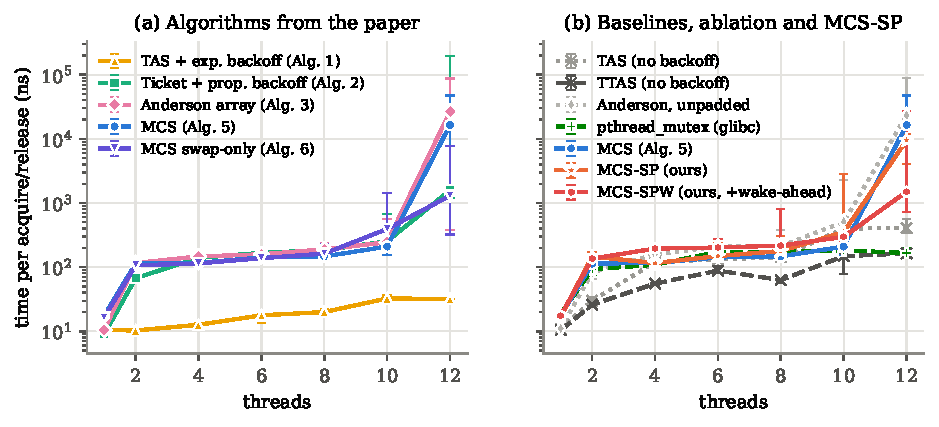
\includegraphics[width=0.92\textwidth]{../figures/fig1_scaling_empty.pdf}
\vspace{-0.6em}
\caption{E1: time per acquire/release pair with an \emph{empty} critical section (paper Figs.~4--6 style; log
scale; lower is better). The queue locks track each other up to 10 threads. Test\_and\_set with backoff is
5--10$\times$ ``faster'' only because it rarely passes the lock to another core (fairness, \S\ref{sec:unfair}).
At 12 threads, the boundary case, every FIFO lock collapses.}
\label{fig:e1}
\end{figure*}

\begin{figure*}[t]\centering
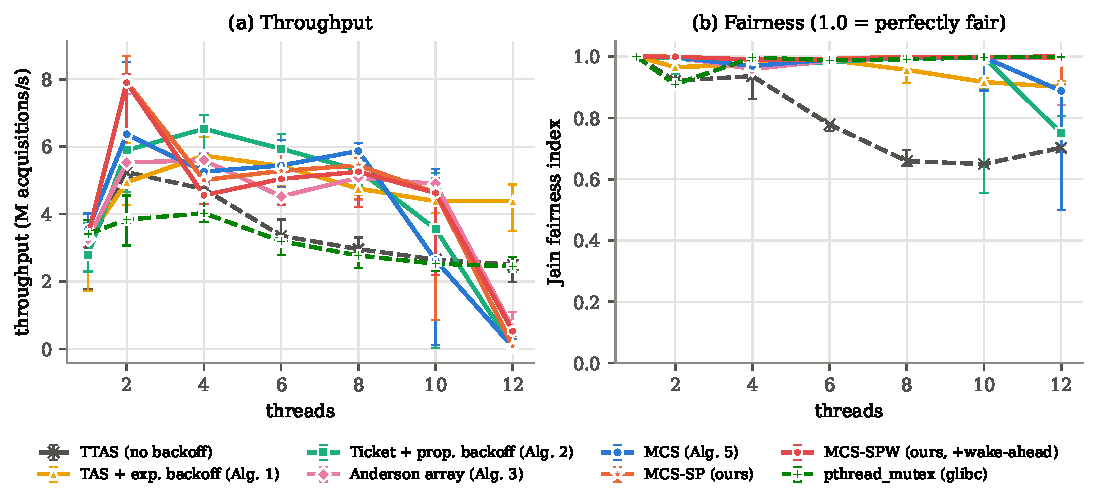
\includegraphics[width=0.92\textwidth]{../figures/fig2_scaling_cs.pdf}
\vspace{-0.6em}
\caption{E2: small critical section plus think time (paper Fig.~7 style). (a) From 2 to 10 threads the
scalable locks deliver comparable throughput, as the paper found. TTAS and glibc's mutex fall behind.
(b) TTAS becomes very unfair. At 12 threads the FIFO locks collapse.}
\label{fig:e2}
\end{figure*}

\subsection{Scaling while threads $\le$ cores: the paper replicates}
With a small critical section (Fig.~\ref{fig:e2}), the four locks the paper calls scalable stay within
4.8--5.9\,M acquisitions/s at 8 threads: MCS 5.87, ticket 5.31, Anderson 5.08, and test\_and\_set with
backoff 4.76. This is the paper's Symmetry result: ``all three of the scalable algorithms have comparable
absolute performance''. Test-and-test\_and\_set degrades to 2.96\,M/s and becomes unfair (Jain 0.66). That
matches the paper's observation that it ``showed the poorest scaling behavior''. glibc's
\texttt{pthread\_mutex} reaches only 2.77\,M/s, about half of MCS, because contended acquisitions go through the
kernel. \mcssp{} stays within 7\% of MCS (5.45\,M/s) and \mcssp{}W within 10\% (5.26\,M/s): when nobody is
preempted, spinning ends before the limit and our extensions cost almost nothing.

Two smaller results. First, the paper's two-processor peak for the swap-only release (Alg.~6) does not
appear: 106\,ns against 113\,ns for MCS at 2 threads. Its ``usurper'' timing window is just a few
instructions wide on a modern core. Second, removing padding from Anderson's lock costs 8--12\% at 4--8
threads (158 vs 147\,ns, 212 vs 189\,ns). At 2 threads it actually \emph{helps} (83 vs 116\,ns), because
both slots then share a line that is already in the right cache.

\subsection{Unfairness masquerading as speed}
\label{sec:unfair}
With an empty critical section (Fig.~\ref{fig:e1}), every FIFO lock needs 110--215\,ns per acquisition at 2--8
threads. That is roughly 2--4 cache-line transfers of about 45\,ns (Table~\ref{tab:calib}): the grant flag,
the lock word or queue tail, and the protected data. Test\_and\_set with backoff needs only 10--20\,ns,
\emph{faster than a single cache-line transfer}. It achieves this by not handing the lock over at all. A
releasing core usually re-acquires before any backed-off waiter retries, so the lock and the data stay in its
L1. Its Jain index at 8 threads is 0.87, and plain TTAS's is 0.24. The paper's metric, average time per
acquisition, cannot see this. On the Symmetry the effect was small; on a modern core, where a hit in the
local cache is roughly 50$\times$ cheaper than a transfer between cores, it dominates. \textbf{Lesson: a lock
benchmark must report fairness next to throughput.}

\begin{figure*}[t]\centering
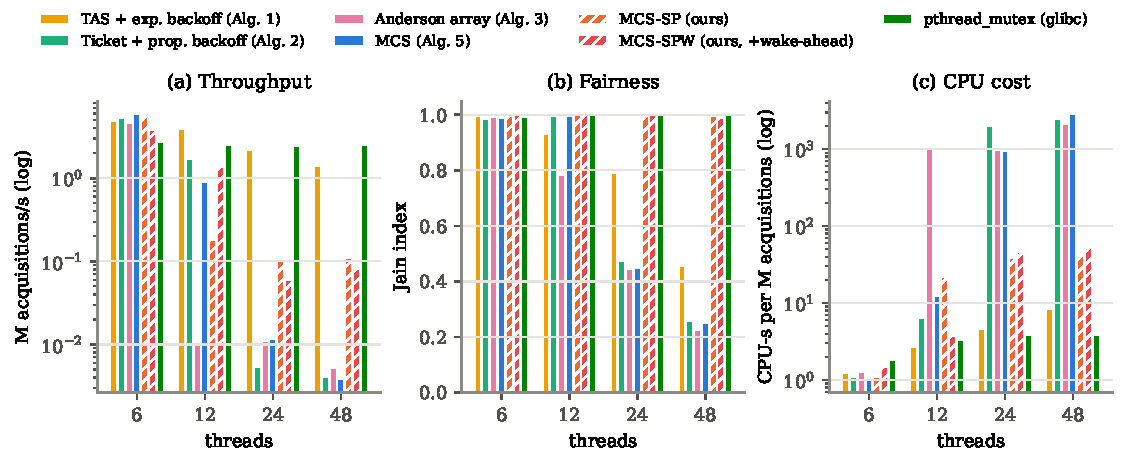
\includegraphics[width=0.95\textwidth]{../figures/fig3_oversub.pdf}
\vspace{-0.6em}
\caption{E3: oversubscription, up to 48 threads on 12 hardware threads (log scales in (a) and (c)). The
paper's FIFO locks lose two to three orders of magnitude of throughput, burn about 1000--2800 CPU-seconds per
million acquisitions, and starve threads. \mcssp{} (hatched) keeps fairness at 0.995 and uses 25--70$\times$
less CPU.}
\label{fig:e3}
\end{figure*}

\subsection{Oversubscription: the FIFO collapse and \mcssp{}}
Fig.~\ref{fig:e3} and Table~\ref{tab:over} show the central result. With 6 threads every lock runs at
2.7--5.9\,M/s. At 24 and 48 threads MCS drops to 0.012 and 0.004\,M/s, which is \textbf{500--1500$\times$
slower}. Ticket and Anderson behave the same way. Fairness also collapses (Jain 0.22--0.47). In one second
the unluckiest thread completed only 1--18 acquisitions, which is practically starvation. Meanwhile the
process burned 950--2850 CPU-seconds per million acquisitions spinning. This is the failure the paper
predicts in \S4.3.

\mcssp{} delivers 0.10--0.11\,M/s at 24 and 48 threads, \textbf{9--29$\times$ more than MCS}. It is
almost perfectly fair (Jain 0.995; the slowest thread still completes 2\,200--4\,200 acquisitions) and uses
\textbf{25--70$\times$ less CPU} (38--41 CPU-s per M). The paper's suggested fallback, test\_and\_set with
backoff, reaches higher throughput (1.4--2.2\,M/s) but is unfair (Jain 0.46--0.79).

\begin{table}[t]\centering\small
\caption{E3 throughput (M acquisitions/s, median of 3). T = threads on 12 hardware threads.}
\label{tab:over}
\setlength\tabcolsep{3.2pt}
\begin{tabular}{@{}rrrrrrrr@{}}\toprule
T & TAS-b & Ticket & Anders. & MCS & SP & SPW & pthr.\\\midrule
6 & 4.82 & 5.37 & 4.65 & \textbf{5.89} & 5.43 & 3.83 & 2.73\\
12 & \textbf{3.90} & 1.72 & 0.01 & 0.89 & 0.18 & 1.38 & 2.50\\
24 & 2.19 & 0.005 & 0.011 & 0.012 & 0.10 & 0.06 & \textbf{2.46}\\
48 & 1.41 & 0.004 & 0.005 & 0.004 & 0.11 & 0.08 & \textbf{2.54}\\\bottomrule
\end{tabular}
\end{table}

\paragraph{The honest comparison: glibc's mutex.} Under heavy oversubscription \texttt{pthread\_mutex}
is still about 23$\times$ faster than \mcssp{} (2.5\,M/s) and is also fair over a one-second window. The
reason is structural, not an implementation defect. glibc's unlock releases the lock and then wakes
\emph{a} waiter, and any thread that happens to be running may take the lock first (``barging''). A strict
FIFO lock must instead wait for the \emph{designated} successor. Once successors are asleep, every hand-off
costs at least one wake-up latency $L$, which bounds throughput at $1/L$. With $L\approx2.5$--$2.8\,\mu$s on
an idle machine, the bound is about 0.36--0.4\,M/s. Under load $L$ grows, and \mcssp{}'s 0.1\,M/s corresponds
to about 10\,$\mu$s per hand-off. The remaining gap is \emph{the price of strict FIFO under preemption}.
\mcssp{} reduces MCS's cost from a time slice per hand-off to a wake-up per hand-off, and it cannot go below
that without giving up FIFO.

\begin{figure}[t]\centering
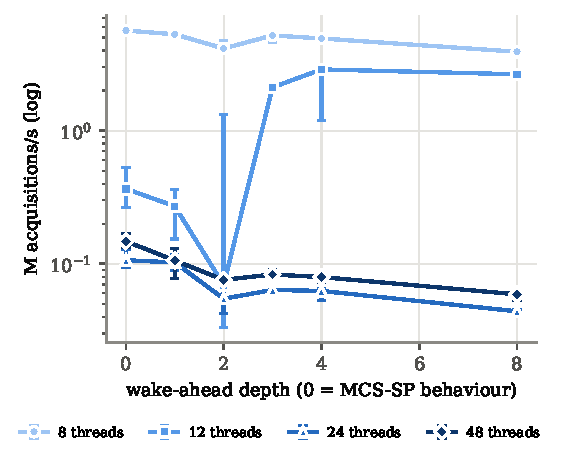
\includegraphics[width=\columnwidth]{../figures/fig6_wake_depth.pdf}
\vspace{-1.6em}
\caption{E7: \mcssp{}W wake-ahead depth. Near the cliff (12 threads), depth $\ge 3$ lifts a strictly FIFO lock
to 2.1--2.9\,M/s, the same range as glibc's mutex. Under heavy oversubscription it hurts.}
\label{fig:e7}
\end{figure}

\subsection{Wake-ahead (\mcssp{}W)}
Wake-ahead attacks that $1/L$ bound by overlapping wake-ups. It helps exactly where we hoped, near the
cliff. At 12 threads \mcssp{}W reaches 1.38\,M/s (E3), against 0.18 for \mcssp{} and 0.89 for MCS. With an empty
CS (E1) it reaches 0.67\,M/s against 0.11 and 0.06, a 6--11$\times$ gain. The depth sweep (Fig.~\ref{fig:e7})
shows that keeping 3--8 waiters awake gives a \emph{stable} 2.1--2.9\,M/s with Jain $=1.00$, which is
glibc-mutex throughput with strict FIFO order. At depth 2 the outcome is bimodal (0.03--1.3\,M/s
across repetitions). Either the pre-woken window absorbs the convoy, or it does not.

Under heavy oversubscription (24--48 threads), wake-ahead \emph{hurts}: 0.06--0.08\,M/s against \mcssp{}'s
0.10--0.11. Each pre-wake adds a system call while the lock is held, and pre-woken waiters spin on CPUs that
the lock holder needs. With threads $\le$ cores it costs 0--25\% depending on depth. Wake-ahead is therefore
a regime-specific tool. Choosing the depth adaptively, from how often waiters actually park, is the obvious
next step (\S\ref{sec:future}).

\begin{figure}[t]\centering
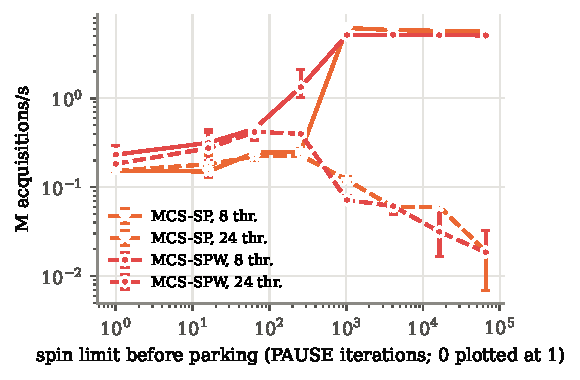
\includegraphics[width=\columnwidth]{../figures/fig4_spin_sweep.pdf}
\vspace{-1.6em}
\caption{E4: spin limit before parking (log--log). With 8 threads (solid), parking too early creates a
self-sustaining convoy, a 25$\times$ cliff between 256 and 1024 \texttt{PAUSE}s. With 24 threads (dashed),
spinning longer steals CPU and the trend reverses.}
\label{fig:e4}
\end{figure}

\subsection{Choosing the spin limit: a convoy model}
Fig.~\ref{fig:e4} shows an unexpectedly sharp cliff. At 8 threads, a spin limit of $\le$256 \texttt{PAUSE}s
gives 0.15--0.25\,M/s, and $\ge$1024 gives 5.1--6.2\,M/s. A simple model explains it. Once any waiter parks
(for example because a background process preempted its predecessor), every later hand-off costs about $L$.
A waiter $k$ places back in the queue then waits about $kL$. If the spin budget is less than $(P{-}1)L$,
every waiter behind also times out and parks, so the convoy \emph{sustains itself}. With $L\approx2.5$--$3\,\mu$s
and $P{-}1=7$, the threshold is about 20\,$\mu$s. 256 \texttt{PAUSE}s last 6--13\,$\mu$s (below it, depending
on P- or E-core), and 1024 last 25--50\,$\mu$s (above it). That is exactly where the cliff is. With 24
threads the regime flips: there is no spare CPU, so spinning longer only delays the threads that need to
run, and shorter limits win (0.15--0.4 against 0.02\,M/s at 65\,536). No single constant is optimal across
regimes. Our default of 1024 favours the common case, threads $\le$ cores. This is the classic
competitive-spinning trade-off~\cite{karlin91}, with one new twist: on a hybrid CPU a ``1024 \texttt{PAUSE}''
budget lasts twice as long on a P-core as on an E-core.

\begin{figure*}[t]\centering
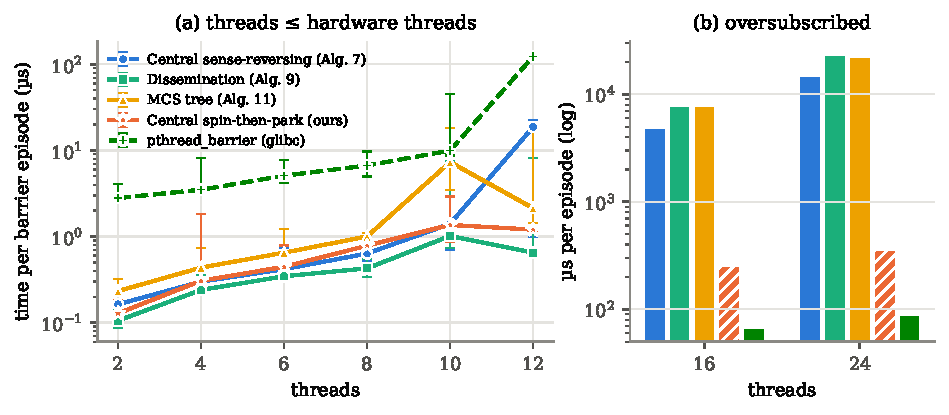
\includegraphics[width=0.88\textwidth]{../figures/fig5_barriers.pdf}
\vspace{-0.6em}
\caption{E5/E6: barriers. (a) The dissemination barrier is fastest on this chip, unlike on the bus-based
Symmetry. (b) When oversubscribed, the paper's spin barriers take 5--23\,ms per episode. Spin-then-park
cuts this 19--66$\times$, and glibc's barrier, which blocks immediately, is fastest.}
\label{fig:bar}
\end{figure*}

\subsection{Barriers}
With $\le$8 threads (Fig.~\ref{fig:bar}a), the dissemination barrier is fastest (0.11--0.43\,$\mu$s per episode),
followed by the centralized barrier (0.16--0.63) and the MCS tree (0.23--1.0). glibc's
\texttt{pthread\_barrier} is 10--25$\times$ slower (2.8--6.7\,$\mu$s), because it sleeps in the kernel.
This \emph{reverses} the paper's Symmetry ranking, where the centralized barrier won and dissemination was
worst for $P>8$ because its $O(P\log P)$ transactions serialized on a single bus. A modern on-chip interconnect
moves lines between \emph{different} pairs of cores in parallel. That is the Butterfly-like property under
which the paper itself predicted dissemination ``will outperform the tree barrier'' (\S5). Our tree
barrier is slower than dissemination for two reasons. Its arrival-then-wake-up critical path is longer,
and our portable version makes children perform an atomic RMW on the parent's word instead of a byte store.

When oversubscribed (Fig.~\ref{fig:bar}b), the spin barriers need 4.9--23\,ms per episode, which is several
scheduler time slices. Our spin-then-park central barrier needs 0.25--0.35\,ms, \textbf{19--66$\times$ faster}.
It matches the plain central barrier with $\le$8 threads, and at 12 it avoids that barrier's collapse (1.2 against
18.7\,$\mu$s). glibc's barrier is faster still (67--89\,$\mu$s), because it blocks immediately instead of
spinning first. That is the same regime trade-off as in Fig.~\ref{fig:e4}.

\section{Discussion}
\paragraph{What survived 35 years.} The core principle, spin locally and end the spin with a single remote
write, is fully confirmed. MCS, ticket and Anderson scale and stay fair while threads $\le$ cores. TTAS
does not. The paper's uncontended-latency ordering still holds. Its warning about preemption was not only
correct, it is the dominant effect on a general-purpose machine.
\paragraph{What changed.} (1) Absolute costs fell by a factor of about 670, but a transfer between cores is
still about 50$\times$ an L1 hit. Locality matters as much as ever. (2) Because of that gap, unfair locks look
5--10$\times$ ``faster'' on the paper's own metric, so fairness must be measured. (3) Point-to-point on-chip
interconnects make the dissemination barrier the winner, as the paper predicted for networks that allow
parallel transactions. (4) Hybrid cores make ``spin $N$ times'' mean different wall-clock times on
different cores. Spin limits should be expressed in time, not iterations. (5) Oversubscription is now
the normal case: browsers, IDEs, thread pools sized above the core count, and hypervisors time-sharing
vCPUs. A lock that assumes one thread per core will meet preemption.
\paragraph{Practical guidance.} If threads $\le$ cores and FIFO matters, use MCS or \mcssp{}, which costs
nothing extra there. If oversubscription is possible and FIFO is not required, a barging futex lock
(glibc) is best. If FIFO is required and the machine runs near saturation, use \mcssp{}W with a small depth.
If FIFO is required and the machine is heavily oversubscribed, use \mcssp{}. It loses to barging locks,
but it avoids MCS's 500--1500$\times$ collapse and starvation.

\section{Threats to validity}
\label{sec:threats}
\textbf{One machine, not isolated.} All data comes from a single laptop with a live desktop session. That is
realistic but noisy, and the 12-thread results are bimodal (for example, Anderson gave 4.0 and 0.009\,M/s in
different repetitions). We report medians with min--max bars, and we draw no conclusions from differences
under about 15\%. \textbf{Turbo and the hybrid scheduler} (Intel Thread Director) affect which core runs which
thread. We did not pin, by design. \textbf{Microbenchmarks only:} we did not test a real application.
\textbf{x86 only:} the C11 orderings are argued in \S\ref{sec:impl} but were not exercised on a weakly
ordered CPU such as Arm, and ThreadSanitizer was unavailable on this machine (\texttt{libtsan} not installed).
Our evidence for correctness is the invariant checks run on every benchmark plus the arguments in
\S\ref{sec:impl} and \S\ref{sec:ext}. \textbf{Coverage:} we did not implement Alg.~4 (Graunke--Thakkar),
Alg.~8 (combining tree) or Alg.~10 (tournament), and a single-socket laptop cannot test NUMA effects.

\section{Future work}
\label{sec:future}
(1) \emph{Adaptive waiting}: express the spin budget in nanoseconds, measure $L$ online, and change both the
spin limit and the wake-ahead depth based on how often waiters actually park. That would choose the right
side of Figs.~\ref{fig:e4} and \ref{fig:e7} automatically. (2) Run on a cloud VM, where the hypervisor
preempts vCPUs \emph{including the lock holder}, and on Arm. (3) Compare with time-published locks~\cite{tp05}
and shuffle locks~\cite{shfl}, and with NUMA cohort locks~\cite{cohort} on a multi-socket server.
(4) Measure a real workload, such as a lock-protected hash table or a memory allocator.

\section{Conclusion}
We re-implemented the spin locks and barriers of Mellor-Crummey and Scott in modern C11 and re-ran their
evaluation on a 2022 hybrid laptop CPU. The paper's central claim holds: local spinning makes
synchronization scale, and MCS is a fair, scalable lock while threads do not outnumber cores. Two new
observations stand out on modern hardware. Unfair locks win the paper's throughput metric by keeping the lock
in one cache, so fairness has to be reported too. And dissemination is the fastest barrier on a chip
whose interconnect moves lines between different cores in parallel. The weakness the paper acknowledged,
preemption of FIFO waiters, turns out to be the dominant effect on a shared machine, where MCS slows down by
up to 1500$\times$. Our extension \mcssp{} adds spin-then-park waiting in about 20 lines. It keeps FIFO order
and MCS's cost when threads $\le$ cores, and it gives 9--29$\times$ the throughput with 25--70$\times$ less CPU
when oversubscribed. Wake-ahead (\mcssp{}W) brings strict FIFO up to glibc-mutex throughput near the
saturation point. Beyond that point, the measured gap to barging locks is the inherent price of strict FIFO under
preemption.

\paragraph{Reproducibility.} Source, raw CSVs and scripts are in the accompanying repository:
\texttt{make \&\& make test \&\& scripts/run\_experiments.sh \&\& uv run --with matplotlib --with pandas
scripts/plot.py}.

\paragraph{Use of AI tools.} As permitted by the course, an AI assistant (Anthropic's Claude) was used
to help implement the code, run the experiments and draft this report. All numbers come from the
included measurements.


\begin{thebibliography}{99}\setlength\itemsep{0pt}\small
\bibitem{mcs91} J.~M. Mellor-Crummey and M.~L. Scott. Algorithms for scalable synchronization on
shared-memory multiprocessors. \emph{ACM Trans.\ Computer Systems}, 9(1):21--65, 1991.
\bibitem{anderson90} T.~E. Anderson. The performance of spin lock alternatives for shared-memory
multiprocessors. \emph{IEEE Trans.\ Parallel and Distributed Systems}, 1(1):6--16, 1990.
\bibitem{gt90} G.~Graunke and S.~Thakkar. Synchronization algorithms for shared-memory multiprocessors.
\emph{IEEE Computer}, 23(6):60--69, 1990.
\bibitem{hfm88} D.~Hensgen, R.~Finkel, and U.~Manber. Two algorithms for barrier synchronization.
\emph{Int.\ J.\ Parallel Programming}, 17(1):1--17, 1988.
\bibitem{amp} M.~Herlihy and N.~Shavit. \emph{The Art of Multiprocessor Programming}. Morgan Kaufmann,
2008 (2nd ed.\ 2020).
\bibitem{qspinlock} J.~Corbet. MCS locks and qspinlocks. \emph{LWN.net}, March 2014.
\bibitem{futex} H.~Franke, R.~Russell, and M.~Kirkwood. Fuss, futexes and furwocks: fast userlevel
locking in Linux. In \emph{Ottawa Linux Symposium}, 2002.
\bibitem{karlin91} A.~R. Karlin, K.~Li, M.~S. Manasse, and S.~Owicki. Empirical studies of competitive
spinning for a shared-memory multiprocessor. In \emph{Proc.\ SOSP}, 1991.
\bibitem{tp05} B.~He, W.~N. Scherer III, and M.~L. Scott. Preemption adaptivity in time-published
queue-based spin locks. In \emph{Proc.\ HiPC}, 2005.
\bibitem{malthusian} D.~Dice. Malthusian locks. In \emph{Proc.\ EuroSys}, 2017.
\bibitem{shfl} S.~Kashyap, I.~Calciu, X.~Cheng, C.~Min, and T.~Kim. Scalable and practical locking with
shuffling. In \emph{Proc.\ SOSP}, 2019.
\bibitem{cohort} D.~Dice, V.~J. Marathe, and N.~Shavit. Lock cohorting: a general technique for designing
NUMA locks. In \emph{Proc.\ PPoPP}, 2012.
\bibitem{nonscalable} S.~Boyd-Wickizer, M.~F. Kaashoek, R.~Morris, and N.~Zeldovich. Non-scalable locks
are dangerous. In \emph{Proc.\ Linux Symposium}, 2012.
\bibitem{jain} R.~Jain, D.-M. Chiu, and W.~Hawe. A quantitative measure of fairness and discrimination for
resource allocation in shared computer systems. DEC Tech.\ Report TR-301, 1984.
\end{thebibliography}
\end{document}
